\documentclass[aspectratio=169]{beamer}

\usetheme{Madrid}
\usecolortheme{seahorse}
\usepackage[utf8]{inputenc}
\usepackage{amsmath}
\usepackage{listings}
\usepackage{xcolor}
\usepackage{graphicx}
\usepackage{booktabs}
\usepackage{tabularx}

\lstdefinestyle{cli}{
  basicstyle=\ttfamily\scriptsize,
  backgroundcolor=\color{black!5},
  frame=single,
  breaklines=true,
  columns=fullflexible,
  keywordstyle=\color{blue},
}
\lstdefinestyle{va}{
  basicstyle=\ttfamily\scriptsize,
  backgroundcolor=\color{black!5},
  frame=single,
  breaklines=true,
  columns=fullflexible,
}
\lstnewenvironment{cli}{\lstset{style=cli}}{}
\lstnewenvironment{va}{\lstset{style=va}}{}

\title{Building openMemristorPDK}
\subtitle{A minimum memristor PDK, built end-to-end with openPDKcreator}
\author{}
\date{}

\begin{document}

\frame{\titlepage}

% ---------------------------------------------------------------
\begin{frame}{Goal}
\begin{itemize}
  \item Build a genuinely \textbf{minimum} PDK for a two-terminal memristor device,
        using \texttt{openPDKcreator}'s own GUI/CLI -- the same tool built and
        hardened over this session against IHP's real SG13G2 PDK.
  \item \textbf{Independent} of that IHP-based project: its own directory,
        its own git history, its own empty starting point -- nothing shared.
  \item Every step documented here, real GUI actions throughout.
  \item Capstone: a real \texttt{openvaf}/\texttt{ngspice} transient
        simulation of the memristor's own compact model, showing the
        classic pinched I-V hysteresis loop.
\end{itemize}
\end{frame}

% ---------------------------------------------------------------
\begin{frame}{Why a fresh copy of the tool, not just a new \texttt{--pdk-root}}
\texttt{openPDKcreator} tracks two different roots:
\begin{itemize}
  \item \texttt{pdk\_root} -- the real (or, here, from-scratch) PDK data
        directory. Freely overridable via \texttt{--pdk-root}.
  \item \texttt{PROJECT\_ROOT} -- where \texttt{library\_index.yaml},
        \texttt{user\_models/}, \texttt{saves/} live. Hard-coded to
        \texttt{Path(\_\_file\_\_).resolve().parents[1]} -- wherever the
        tool's own code physically sits. \textbf{Not} a CLI flag.
\end{itemize}
\vspace{0.5em}
For genuine independence, the tool itself was copied into a new home:
\begin{cli}
cd openPDKcreator
cp -r openpdkcreator main.py LICENSE openMemristorPDK/
mkdir -p openMemristorPDK/data/openmemristorpdk
cd openMemristorPDK && git init
\end{cli}
Reachable inside the already-running container at
\texttt{/foss/designs/openMemristorPDK/} -- no new container/mount needed.
\end{frame}

% ---------------------------------------------------------------
\begin{frame}{Launching against the new, empty project}
\begin{cli}
python3 main.py --pdk-root data/openmemristorpdk inventory
> Nothing found -- has ihp/fetch.py been run yet?

python3 main.py --pdk-root data/openmemristorpdk gui
\end{cli}
\vspace{0.5em}
Honest, real output for a genuinely empty deck -- confirming
\texttt{openPDKcreator} really does support building up from nothing,
not just editing an existing real PDK.
\end{frame}

% ---------------------------------------------------------------
\begin{frame}{The PDK Wizard's own Analog/Memristor path}
\begin{center}
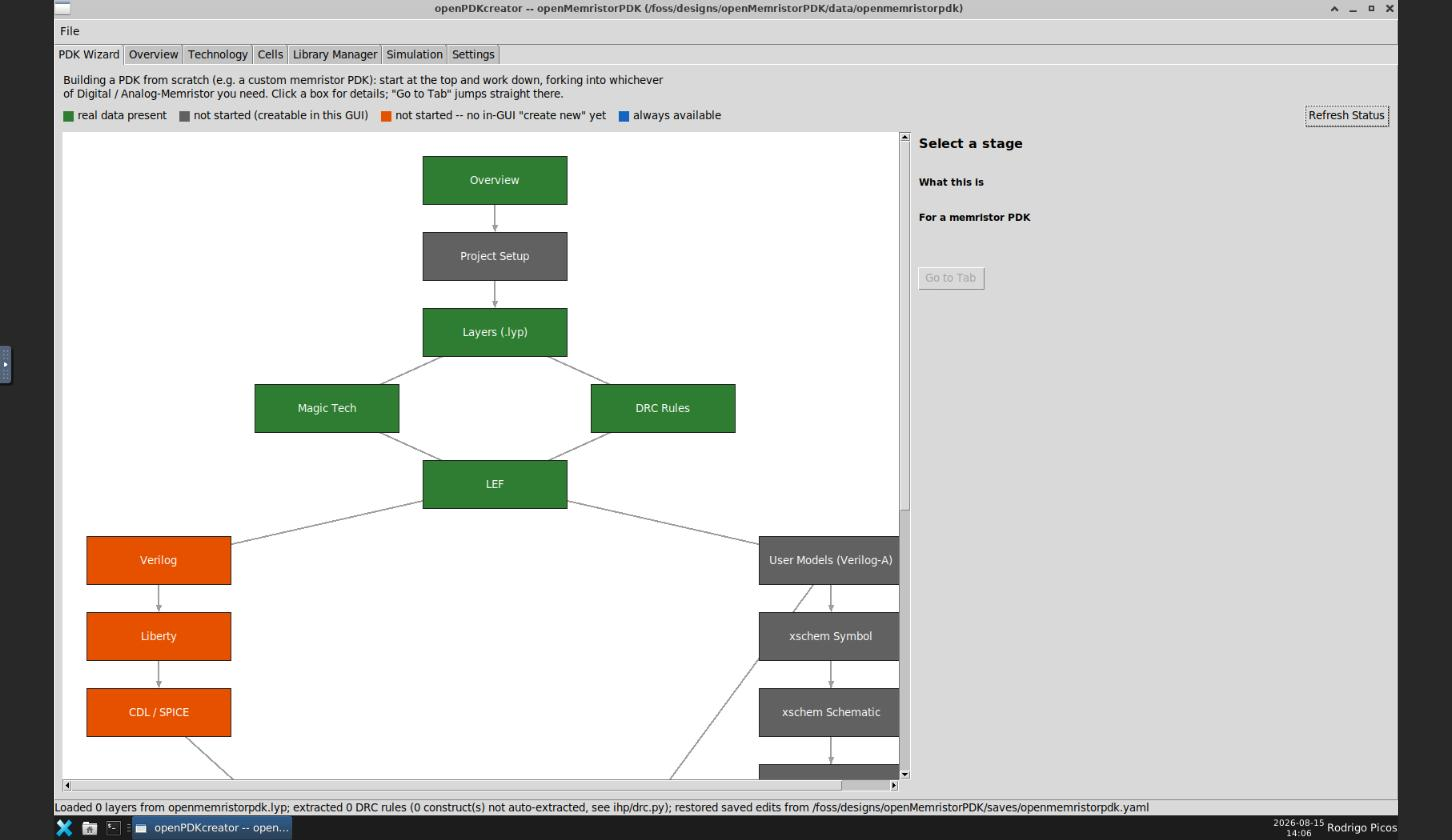
\includegraphics[width=0.65\textwidth]{figures/pdk_wizard.jpg}
\end{center}
\footnotesize
Green = real data present. The wizard already forks
Digital vs. Analog/Memristor -- this walk follows the right-hand fork:
Layers $\to$ Magic Tech / DRC $\to$ LEF $\to$ User Models (Verilog-A)
$\to$ xschem Symbol/Schematic.
\end{frame}

% ---------------------------------------------------------------
\begin{frame}{Layers: a 4-layer memristor stack}
Technology $\to$ Layers $\to$ \textbf{New .lyp File...}, then
\textbf{New Layer} $\times 4$:
\begin{center}
\begin{tabularx}{\textwidth}{lccX}
\toprule
Name & GDS layer/dt & Purpose & Role \\
\midrule
BE & 30/0 & drawing & Bottom electrode metal \\
MEM & 31/0 & drawing & Memristive switching oxide \\
TE & 32/0 & drawing & Top electrode metal \\
PRBOUNDARY & 235/4 & marker & Cell outline, no real geometry \\
\bottomrule
\end{tabularx}
\end{center}
\vspace{0.3em}
\footnotesize
Fictional, illustrative GDS numbers/colors -- this is a demo stack, not a
qualified process. Exported via File $\to$ \textbf{Export Edited Layers}
to \texttt{export/openmemristorpdk/libs.tech/klayout/tech/*.lyp}, a real,
valid, open\_pdks-format KLayout layer file.
\end{frame}

% ---------------------------------------------------------------
\begin{frame}{Magic Tech + DRC Rules}
\begin{columns}
\column{0.5\textwidth}
\textbf{Magic Tech} (Technology $\to$ Magic Tech):
\begin{itemize}
  \item \textbf{New .tech File...}
  \item 1 real plane: \texttt{metal}
  \item 3 real types: \texttt{be}, \texttt{mem}, \texttt{te}
\end{itemize}
\column{0.5\textwidth}
\textbf{DRC Rules} (Technology $\to$ DRC Rules):
\begin{itemize}
  \item \textbf{New DRC Deck...}, \textbf{New Rule}
  \item \texttt{MEM.W.1}: minimum width, 0.1\,\textmu m
\end{itemize}
\end{columns}
\vspace{0.5em}
Both exported via File $\to$ \textbf{Save Edits} / \textbf{Export Edited
Magic Types} / \textbf{Export Edited DRC Rules}.
\end{frame}

% ---------------------------------------------------------------
\begin{frame}{Library Manager: the real payoff}
\begin{center}
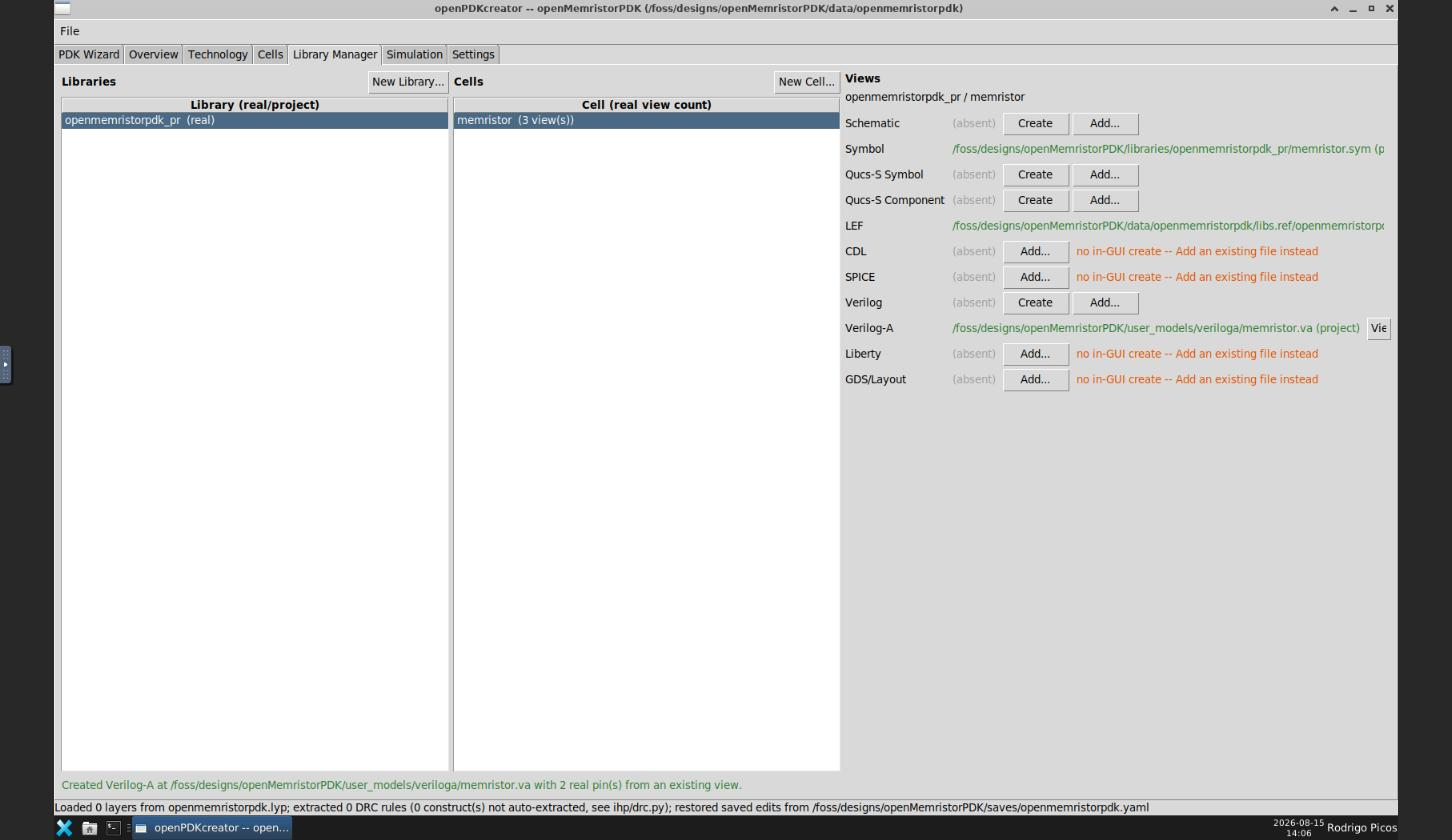
\includegraphics[width=0.65\textwidth]{figures/library_manager.jpg}
\end{center}
\end{frame}

% ---------------------------------------------------------------
\begin{frame}{Library Manager: what actually happened}
\begin{enumerate}
  \item The real LEF macro is auto-discovered: library
        \texttt{openmemristorpdk\_pr}, cell \texttt{memristor}, 1 view.
  \item \textbf{Create} $\to$ Symbol: a real, valid xschem \texttt{.sym}
        skeleton at \texttt{libraries/openmemristorpdk\_pr/memristor.sym}.
  \item \textbf{Create} $\to$ Verilog-A:
\begin{quote}
\ttfamily\small
Created Verilog-A at .../user\_models/veriloga/memristor.va
with 2 real pin(s) from an existing view.
\end{quote}
\end{enumerate}
\medskip
The real pins (\texttt{BE}, \texttt{TE}, both \texttt{INOUT} from the
LEF) were pulled straight into the generated
\texttt{module memristor(BE, TE);} -- \texttt{infer\_ports\_for\_cell}'s
LEF $\to$ xschem $\to$ existing-Verilog priority, validated end to end on
a brand-new project it had never seen before.
\end{frame}

% ---------------------------------------------------------------
\begin{frame}{The generated Verilog-A model}
\begin{center}
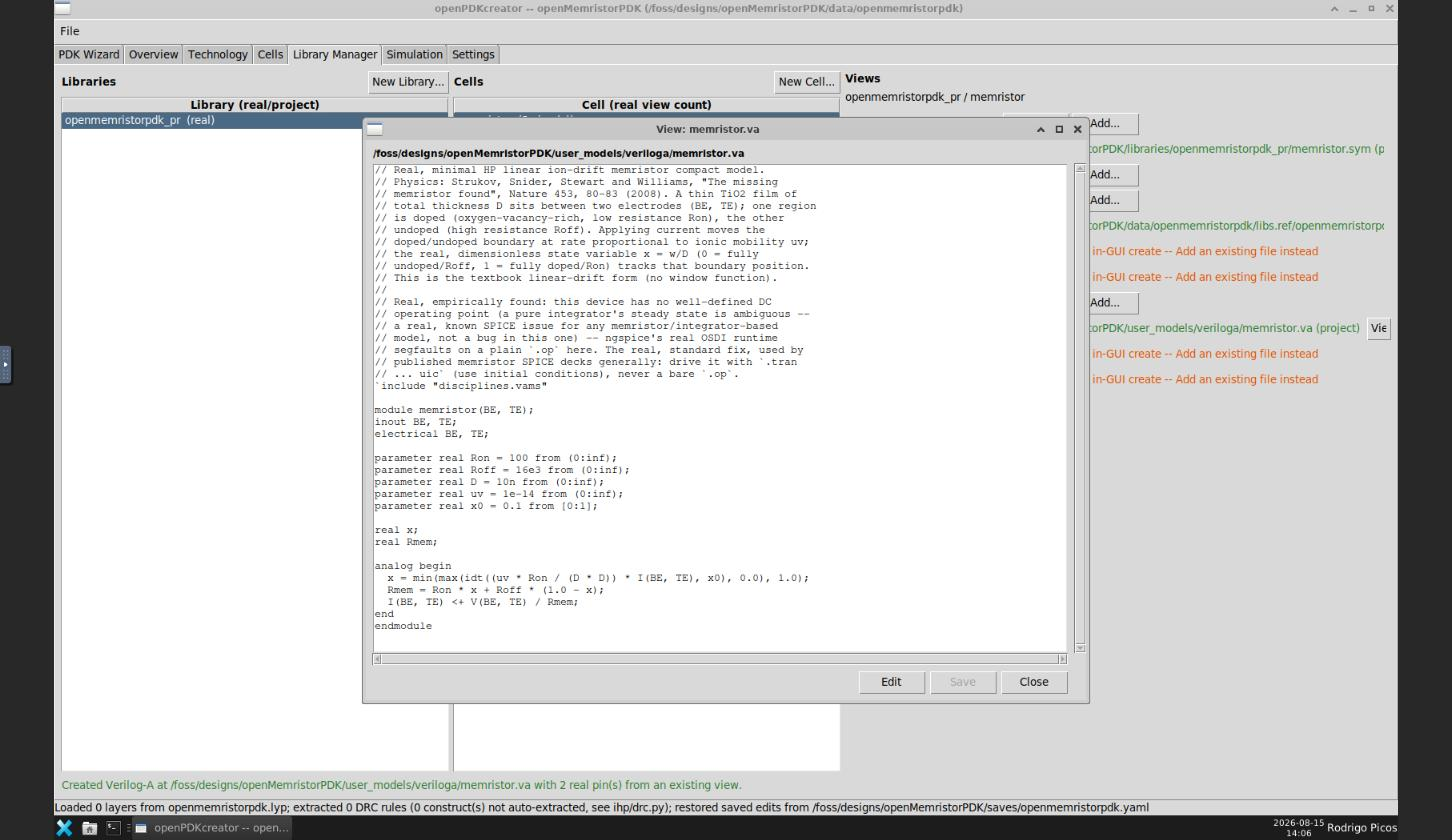
\includegraphics[width=0.65\textwidth]{figures/veriloga_model.jpg}
\end{center}
\end{frame}

% ---------------------------------------------------------------
\begin{frame}{The physics: HP linear ion-drift memristor}
Strukov, Snider, Stewart \& Williams, \emph{``The missing memristor
found''}, Nature 453, 80--83 (2008).
\begin{itemize}
  \item A thin oxide film of thickness $D$ between two electrodes
        (BE, TE); one region doped (low resistance $R_{on}$), the
        other undoped ($R_{off}$).
  \item State $x = w/D \in [0,1]$: the doped/undoped boundary
        position.
  \item[] $\displaystyle \frac{dx}{dt} = \frac{\mu_v R_{on}}{D^2}\, i(t)$
  \item[] $\displaystyle R_{mem}(x) = R_{on}\,x + R_{off}\,(1-x)$
  \item[] $\displaystyle v = R_{mem}(x)\, i$
\end{itemize}
\vspace{0.3em}
Textbook linear-drift form -- no window function. The template the
Library Manager generated was replaced with this real physics,
implemented via Verilog-A's \texttt{idt()} (the state's own integral,
seeded at $x_0$).
\end{frame}

% ---------------------------------------------------------------
\begin{frame}[fragile]{Compiling and instantiating it -- real gotchas found}
\begin{cli}
openvaf memristor.va --output memristor.osdi   # compiles clean
\end{cli}
Getting it to actually \emph{run} in ngspice surfaced three real,
empirically-found issues, none of them documented anywhere obvious:
\begin{enumerate}
  \item \textbf{Name collision}: ngspice ships its own built-in XSPICE
        \texttt{memristor} model. A Verilog-A module of the same name
        silently binds to the wrong one and segfaults. Fixed by
        renaming the simulation-only copy to \texttt{hp\_memristor}
        (the PDK's own cell/file keep the name \texttt{memristor}).
  \item \textbf{Load order}: \texttt{osdi file.osdi} inside a
        \texttt{.control} block runs \emph{after} \texttt{.model} cards
        are parsed. It must be pre-loaded via a \texttt{.spiceinit} in
        the working directory -- exactly IHP's own real convention.
  \item \textbf{Device letter}: OSDI compact models instantiate with
        the \texttt{N} prefix (\texttt{n1 te 0 modelname}), not
        XSPICE's \texttt{a}. Confirmed by reverse-engineering a real
        IHP resistor subcircuit (\texttt{NR1 ... res\_rppd}).
  \item Model parameters (\texttt{ron}, \texttt{roff}, ...) belong on
        the \texttt{.model} card, not the instance line.
\end{enumerate}
\end{frame}

% ---------------------------------------------------------------
\begin{frame}[fragile]{The real testbench}
\begin{va}
.model mm hp_memristor ron=100 roff=16k d=10n uv=1e-14 x0=0.3
n1 te 0 mm
vte te 0 dc 0 sin(0 1.0 0.6)
.tran 300u 3.34
.control
  run
  wrdata memristor_tran.csv v(te) i(vte)
.endc
\end{va}
A 1\,V, 0.6\,Hz sine drive across the device, 2 real periods, run via:
\begin{cli}
bash run_simulation.sh
# [1/3] openvaf hp_memristor.va --output hp_memristor.osdi
# [2/3] ngspice -b mem_tran.sp
# [3/3] python3 plot_memristor.py
\end{cli}
\end{frame}

% ---------------------------------------------------------------
\begin{frame}{Result: the real pinched hysteresis loop}
\begin{center}
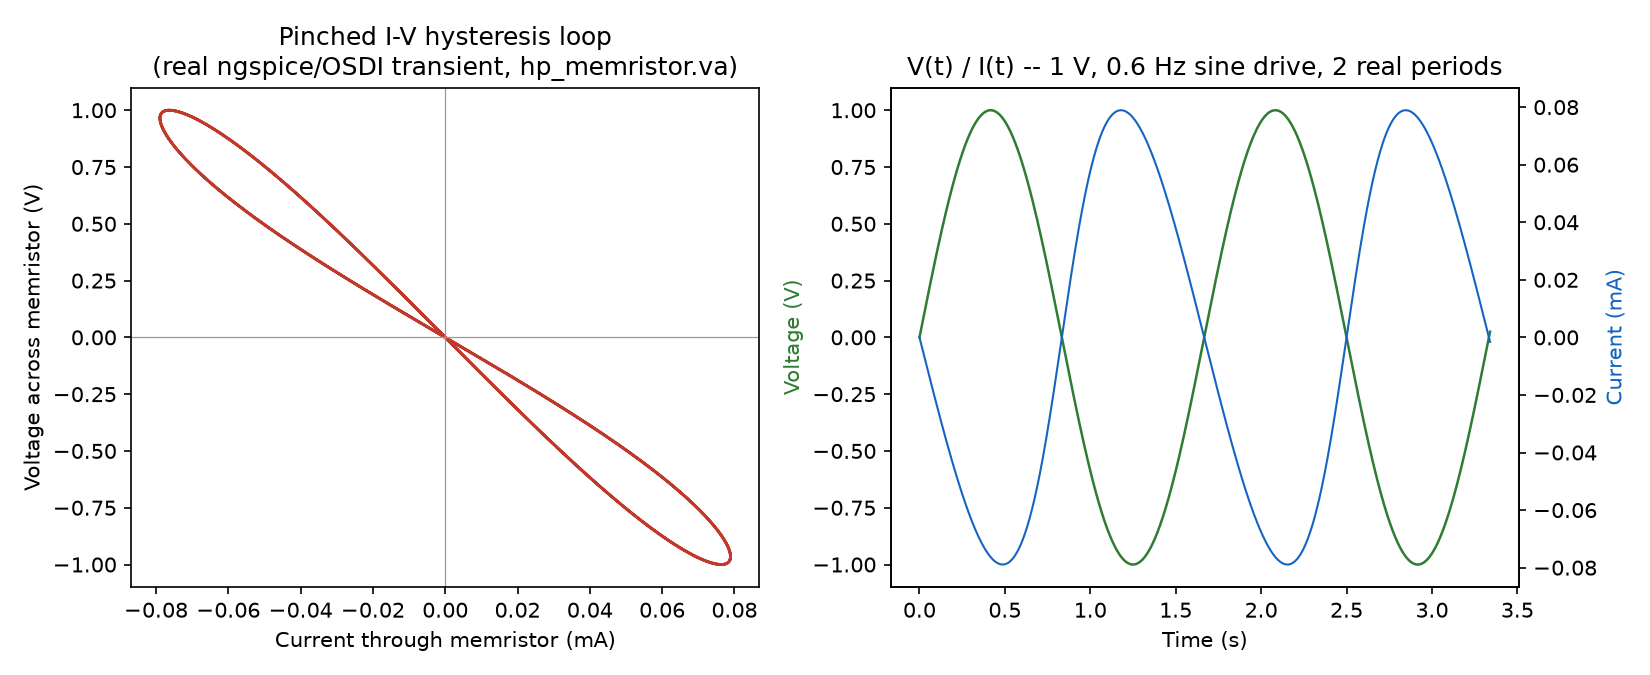
\includegraphics[width=0.65\textwidth]{figures/memristor_transient.png}
\end{center}
\footnotesize
Real, simulated data (11{,}145 points) -- the I-V loop pinches exactly
at the origin every half-cycle, the defining fingerprint of a
memristor: at $V{=}0$, $I{=}0$ always, regardless of history, while the
loop's two branches show a genuinely different resistance depending on
which way the state $x$ was last driven.
\end{frame}

% ---------------------------------------------------------------
\begin{frame}{What's real here}
\begin{itemize}
  \item Independent project, own git history
  \item 4-layer stack, exported \texttt{.lyp}
  \item Magic tech planes/types
  \item 1 DRC rule (unbound layer)
  \item LEF macro, 2 real pins
  \item xschem symbol
  \item Verilog-A model, real physics
  \item Real \texttt{openvaf} compile
  \item Real \texttt{ngspice} transient
\end{itemize}
{\scriptsize See \texttt{walkthrough\_full.tex} for the current,
complete state.}
\end{frame}

% ---------------------------------------------------------------
\begin{frame}{Where everything lives}
\begin{cli}
openMemristorPDK/
  data/openmemristorpdk/        # the live, editable PDK tree
  export/openmemristorpdk/      # real, open_pdks-format output
  libraries/openmemristorpdk_pr/memristor.sym
  user_models/veriloga/memristor.va   # real physics, real pins
  docs/simulation/
    hp_memristor.va             # renamed copy, for ngspice
    mem_tran.sp  run_simulation.sh  plot_memristor.py
    memristor_transient.png
  saves/openmemristorpdk.yaml   # Magic Types + DRC edits
\end{cli}
\end{frame}

\begin{frame}
\centering\Large Thanks!
\end{frame}

\end{document}
